\documentclass{beamer}
\usepackage[T1]{fontenc}
\usepackage[utf8]{inputenc}
\usepackage{listings}
\usepackage{caption}
\usepackage{amssymb}
\usepackage{upgreek}
\usepackage{mathtools}
\usepackage{graphicx}
\graphicspath{ {./images/} }
\usepackage{tikz}
\usetikzlibrary{shapes.callouts,shadows, calc}

\usepackage{color}
\definecolor{keywordcolor}{rgb}{0.7, 0.1, 0.1}   % red
\definecolor{commentcolor}{rgb}{0.4, 0.4, 0.4}   % grey
\definecolor{symbolcolor}{rgb}{0.0, 0.1, 0.6}    % blue
\definecolor{sortcolor}{rgb}{0.1, 0.5, 0.1}      % green
\definecolor{errorcolor}{rgb}{1, 0, 0}           % bright red
\definecolor{stringcolor}{rgb}{0.5, 0.3, 0.2}    % brown

\def\lstlanguagefiles{lstlean.tex}
% set default language
\lstset{language=lean}

\usetheme[compress]{Berlin}
\usecolortheme{default}

\input{thesis_macros}

\captionsetup{labelformat=empty}

%Information to be included in the title page:
\title{An Introduction to Differential Geometry and Collar Neighbourhoods}
\author{Hannah Scholz}
\institute[MI]{Mathematical Institute of the University of Bonn}
\date{11.06.2026}



\begin{document}

\frame{\titlepage}

\section{Understanding the Statement}

\begin{frame}{Collar Neighbourhood}
\begin{block}{Definition: Collar Neighbourhood}
  Let $M$ be a \alert<2,3>{smooth manifold with boundary}. 
  Let $U$ be a neighbourhood of the boundary $\boundary M$. 
  $U$ is called a \emph{collar neighbourhood} if there is a \alert<3>{diffeomorphism} $\varphi \colon \boundary M \times [0, 1) \to U$ 
  such that $\varphi (p, 0) = p$ for all $p \in M$. 
\end{block}
\begin{figure}
\begin{minipage}[b]{0.9\linewidth}
  \centering
  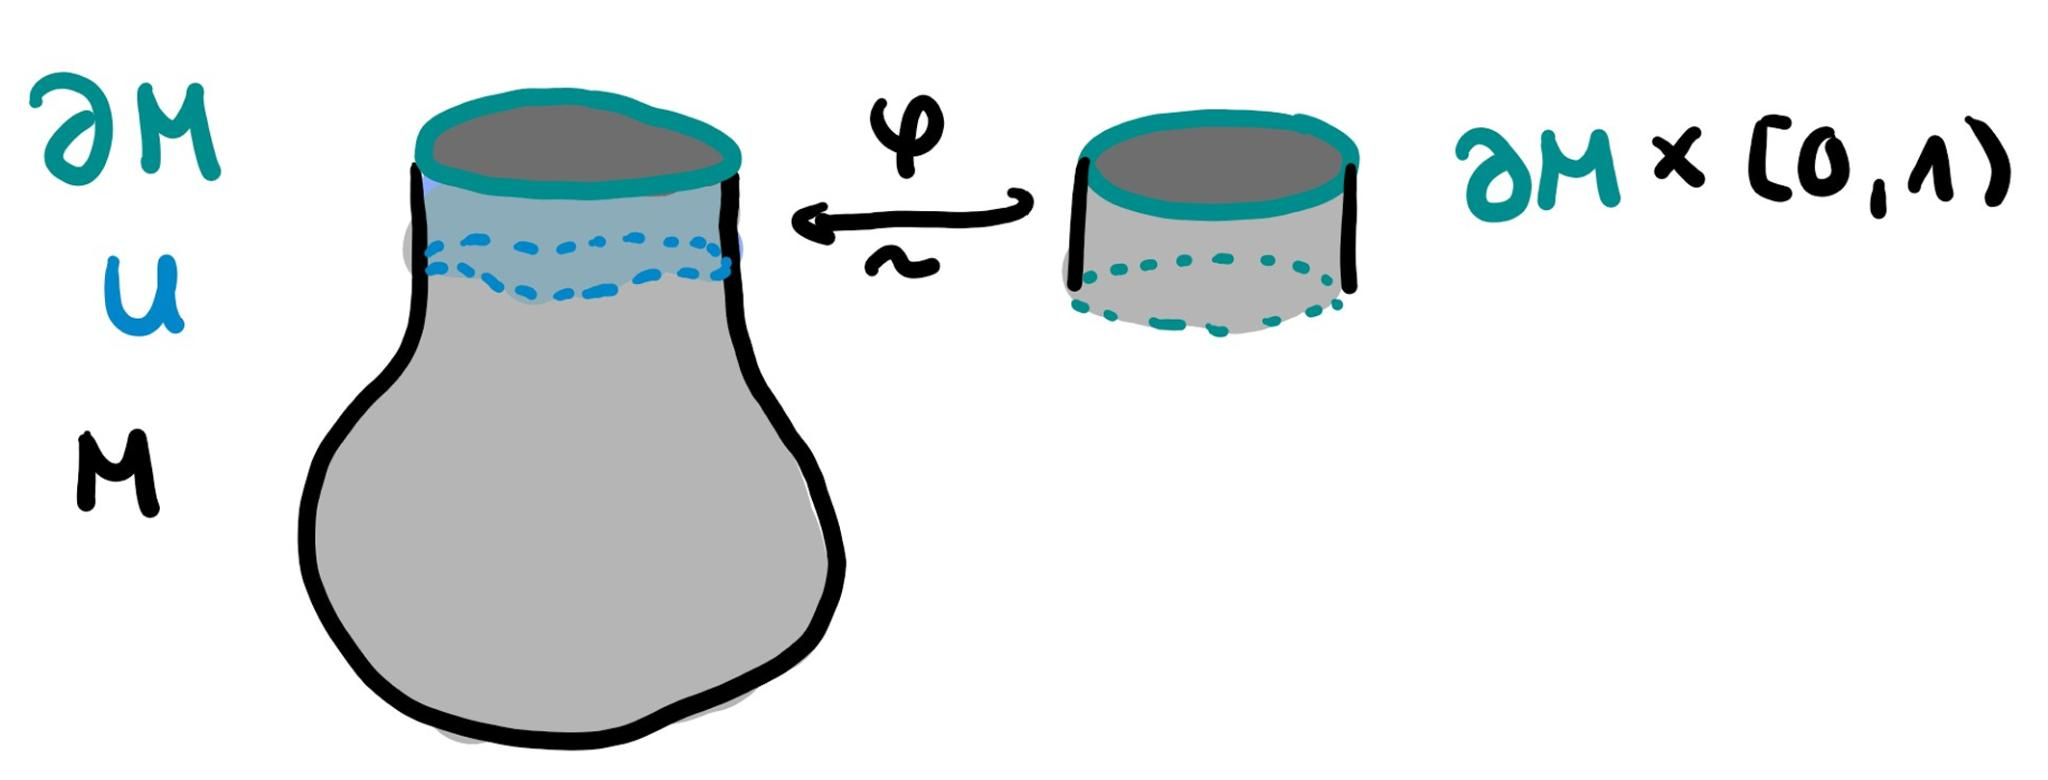
\includegraphics[width=\textwidth]{images/collarneighborhood.png}
  \caption{A collar neighbourhood}
\end{minipage}
\end{figure}
\end{frame}

\begin{frame}{Collar Neighbourhood Theorem}
\begin{block}{Collar Neighbourhood Theorem}
  Let $M$ be a smooth manifold with non-empty boundary. 
  Then $\boundary M$ has a collar neighbourhood.
\end{block}
\end{frame}

\begin{frame}{Topological Manifold with Boundary}
\setbeamertemplate{enumerate items}[default]
%\small
\begin{block}{Definition: Topological Manifold with Boundary}
  A topological space $M$ is a \emph{topological $n$-manifold} if
  \begin{enumerate}[(i)]
    %\setlength{\itemsep}{0pt}
    \item $M$ is Hausdorff.
    \item $M$ is second-countable, i.e.\ $M$ has a countable base.
    \item $M$ is locally Euclidean, i.e.\ for every point $p$ there is a neighbourhood of $p$ that is homeomorphic to an open set in $\bH^n$.
  \end{enumerate}
\end{block}
\begin{block}{Definition: Chart}
Let $M$ be a topological manifold with boundary. 
Let $U$ be an open subset of $M$ and $\varphi \colon U \to \bH^n$ a homeomorphism onto an open subset of $\bH^n$. 
Then we call $(U, \varphi)$ a chart of $M$. 
\end{block}
\end{frame}

\begin{frame}{Boundary of a Topological Manifold}
\setbeamertemplate{enumerate items}[default]
\begin{block}{Definition: Boundary}
Let $M$ be a topological manifold with boundary. 
\begin{enumerate}[(i)]
  \item A point $p \in M$ is a \emph{boundary point} if it is in the domain of a \emph{boundary chart}, i.e.\ a chart $(U, \varphi)$ with $\varphi(p) \in \boundary \bH^n$. 
  \item A point $p \in M$ is an \emph{interior point} if it is in the domain of an \emph{interior chart}, i.e.\ a chart $(U, \varphi)$ with $\varphi(U) \cap \boundary \bH^n = \varnothing$. 
\end{enumerate}
\end{block}
\begin{figure}
\begin{minipage}[b]{0.8\linewidth}
  \centering
  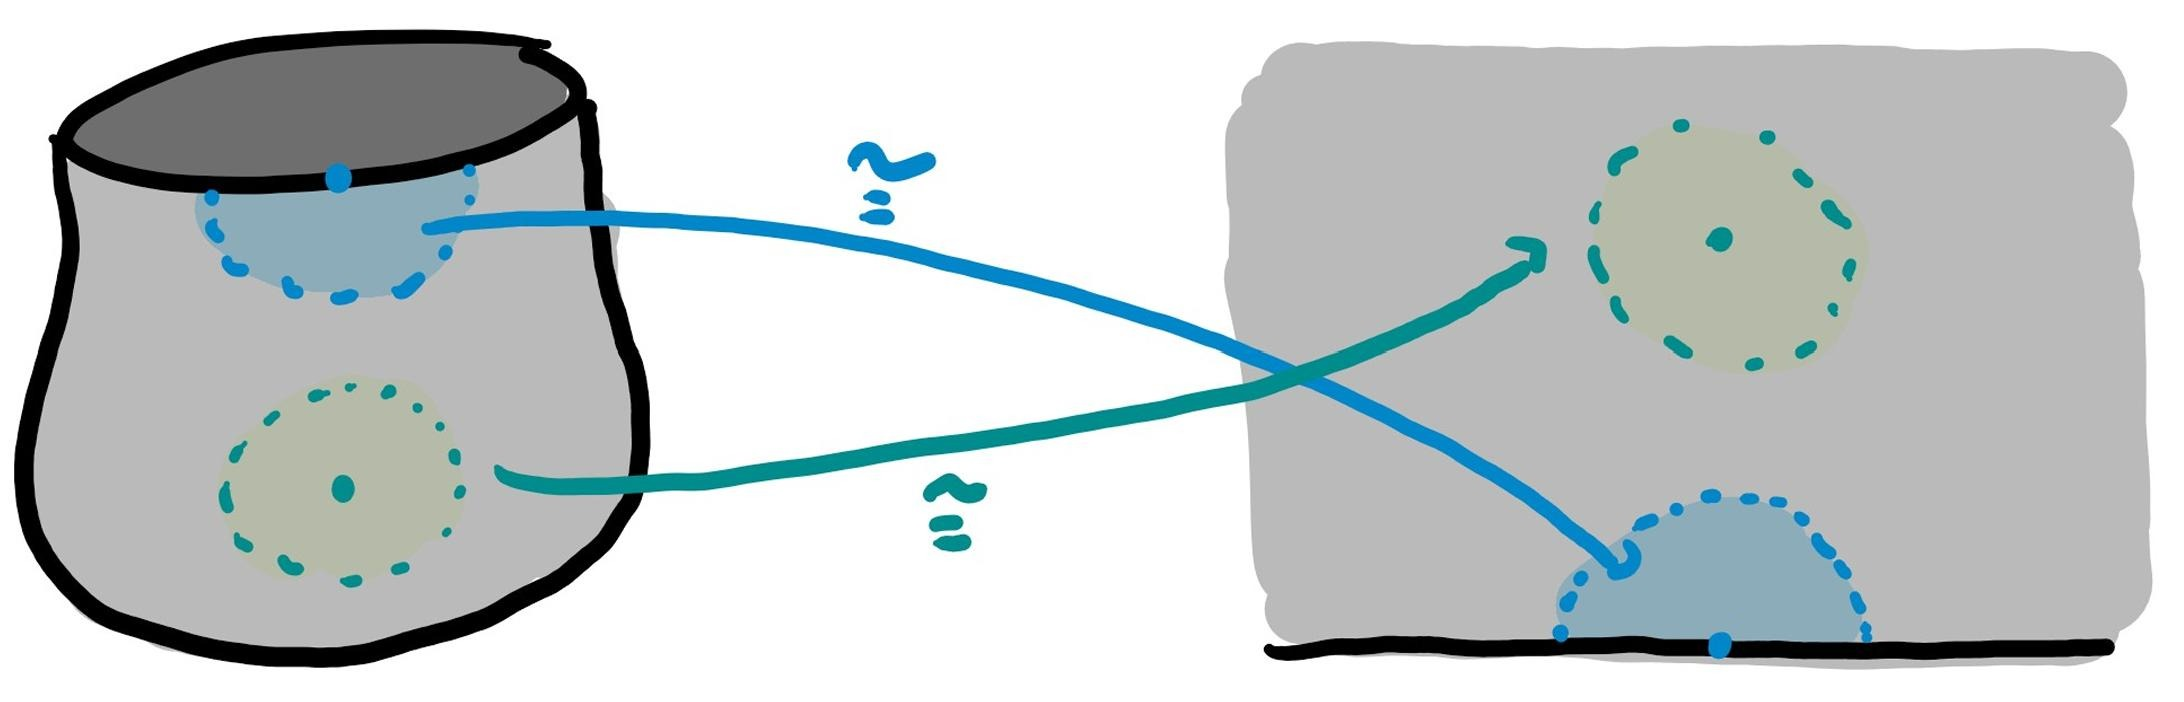
\includegraphics[width=\textwidth]{images/topologicalmanifold.png}
  %\caption{Topological manifold with a boundary and interior chart}
\end{minipage}
\end{figure}
\end{frame}

\begin{frame}{Smooth Manifold}
\begin{block}{Definition: Smooth Atlas}
Let $M$ be a topological manifold. 
Let $\fA$ be a collection of charts whose domains cover $M$.
$\fA$ is a smooth atlas for $M$ if any two charts $(\varphi, U)$ and $(\psi, V)$ are \emph{smoothly compatible}, i.e.\ either $U \cap V$ is empty or $\psi \circ \inv{\varphi} \colon \varphi(U \cap V) \to \psi (U \cap V)$ is smooth in the ordinary sense.
\end{block}
\begin{block}{Definition: Smooth Manifold}
A pair $(M, \fA)$ of a topological manifold $M$ and a smooth altas $\fA$ on $M$, which is maximal with respect to inclusion, is called a \emph{smooth manifold}. 
\end{block}
\end{frame}

\begin{frame}{Compatible Charts}
\begin{figure}
\begin{minipage}[b]{0.7\linewidth}
  \centering
  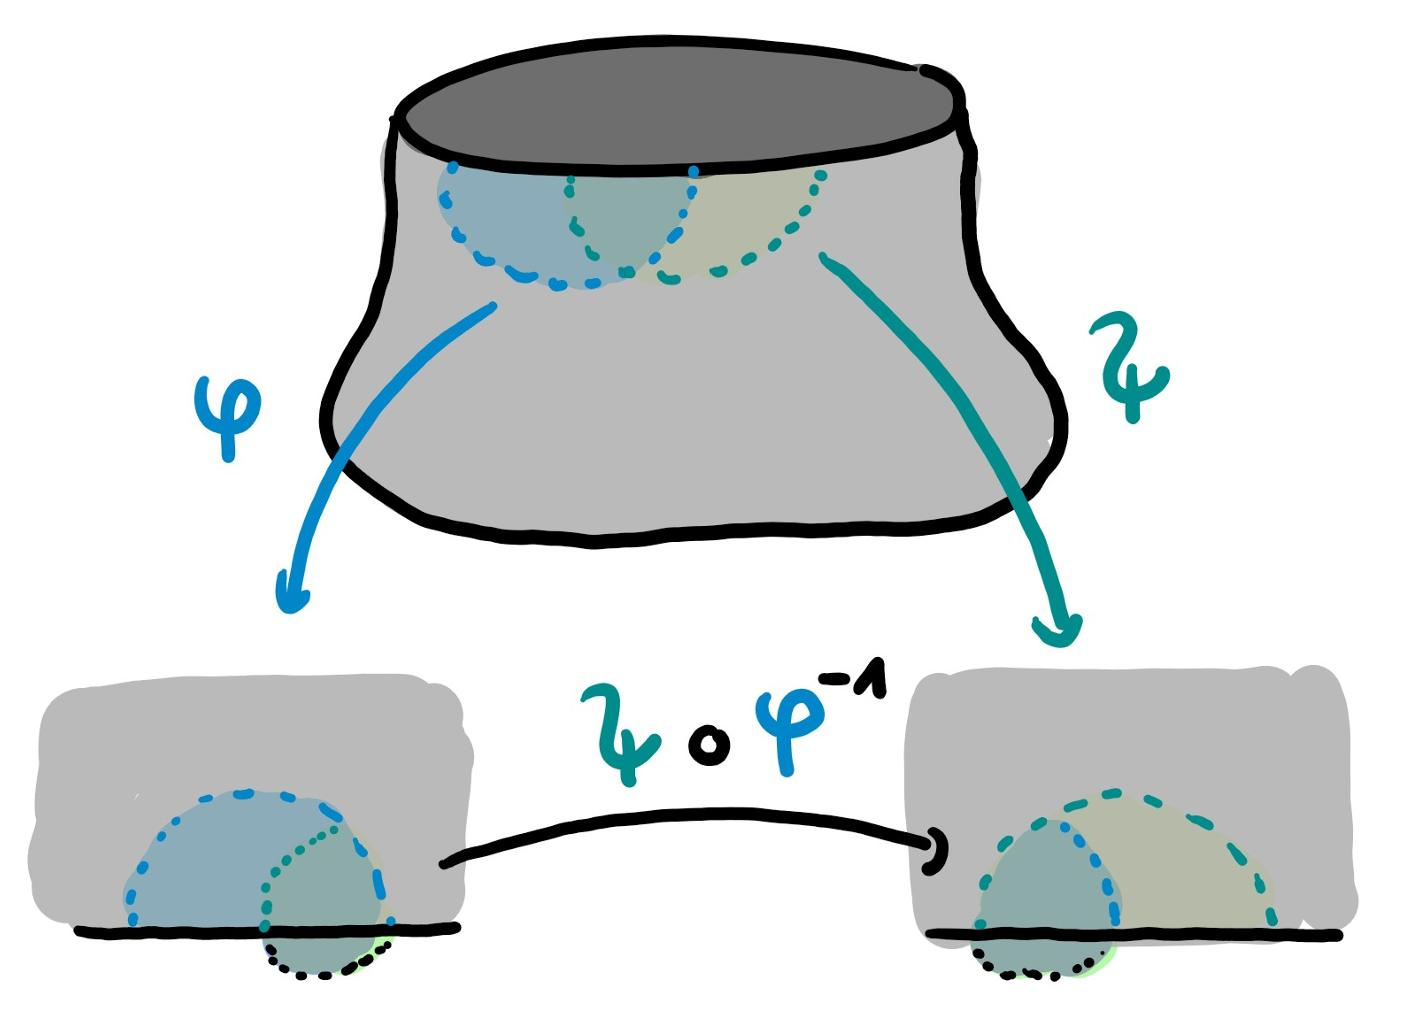
\includegraphics[width=\textwidth]{images/compatiblecharts.png}
  \caption{Compatibility of charts}
\end{minipage}
\end{figure}
\end{frame}

\begin{frame}{Smooth Maps}
\begin{block}{Defintion: Smooth Map}
Let $(M, \fA_M)$ and $(N, \fA_N)$ be smooth manifolds. 
A map $F \colon M \to N$ is called \emph{smooth} if for each $p \in M$ there are charts $(U, \varphi) \in \fA_M$ and $(V, \psi) \in \fA_N$ such that $p \in U$, $F(p) \in U$ and $\psi \circ F \circ \inv{\varphi} \colon \varphi(U) \to \psi(V)$ is smooth. 
\end{block}
\begin{block}{Definition: Diffeomorphism}
A \emph{diffeomorphism} between two smooth manifolds $(M, \fA_M)$ and $(N, \fA_N)$ is a smooth bijective map that has a smooth inverse.
\end{block}
\end{frame}

\begin{frame}{Smooth Maps}
\begin{figure}
\begin{minipage}[b]{0.7\linewidth}
  \centering
  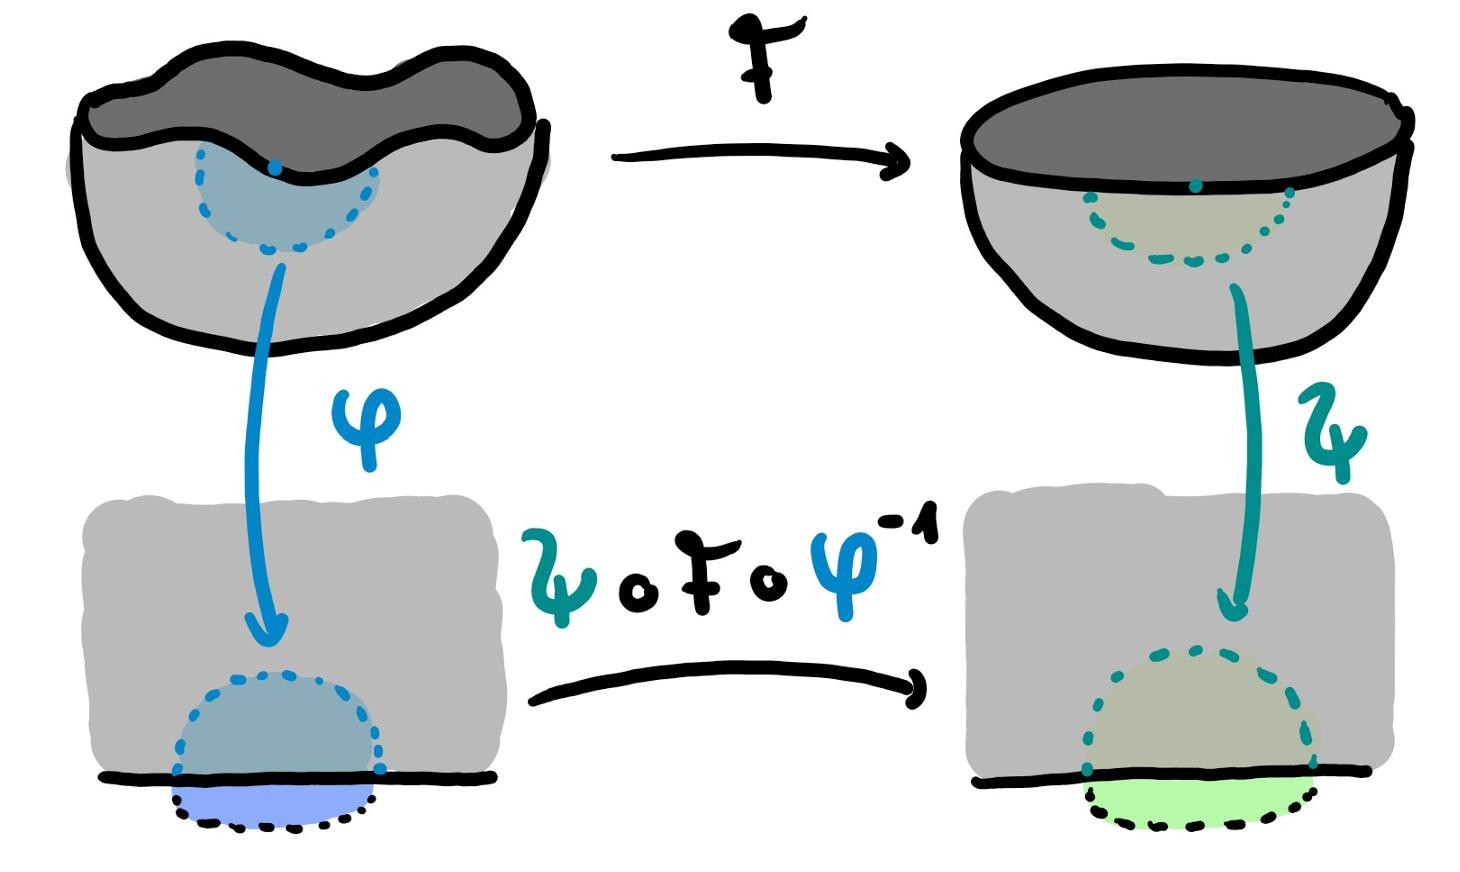
\includegraphics[width=\textwidth]{images/smoothmap.png}
  \caption{Local Smoothness}
\end{minipage}
\end{figure}
\end{frame}

\begin{frame}{Collar Neighbourhoods}
\begin{block}{Definition: Collar Neighbourhood}
  Let $M$ be a {smooth manifold with boundary}. 
  Let $U$ be a neighbourhood of the boundary $\boundary M$. 
  $U$ is called a \emph{collar neighbourhood} if there is a {diffeomorphism} $\varphi \colon \boundary M \times [0, 1) \to U$ 
  such that $\varphi (p, 0) = p$ for all $p \in M$. 
\end{block}
\begin{block}{Collar Neighbourhood Theorem}
  Let $M$ be a smooth manifold with non-empty boundary. 
  Then $\boundary M$ has a collar neighbourhood.
\end{block}
\end{frame}

\section{Understanding the Motivation}

\begin{frame}{Cobordism}
\begin{block}{Definition: Cobordism}
Smooth manifolds $M$ and $N$ are called \emph{cobordant} if there is a compact smooth manifold $W$ such that $\boundary W$ is diffeomorphic to $M \sqcup N$. 
\end{block}
\begin{block}{Lemma}
Cobordism is an equivalence relation.
\end{block}
\end{frame}

\begin{frame}{Transitivity of Cobordism}
\begin{figure}
\begin{minipage}[b]{0.9\linewidth}
  \centering
  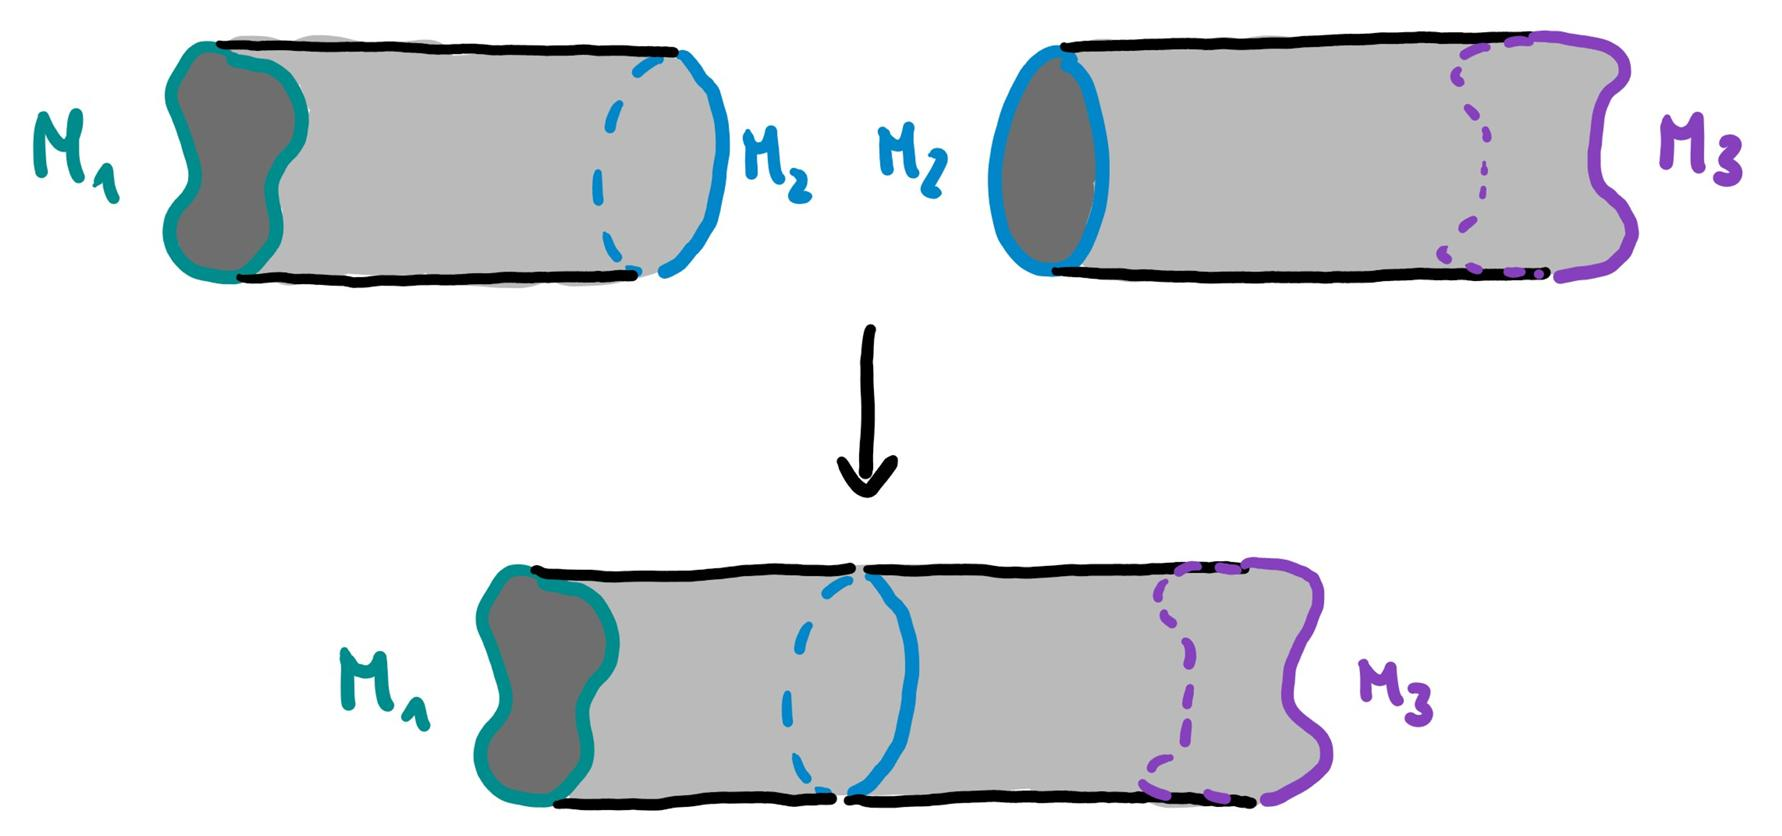
\includegraphics[width=\textwidth]{images/transitivitycobordism.png}
  \caption{Transitivity of Cobordism}
\end{minipage}
\end{figure}
\end{frame}

\begin{frame}{Glueing along Boundary: The Problem}
\begin{figure}
\begin{minipage}[b]{0.9\linewidth}
  \centering
  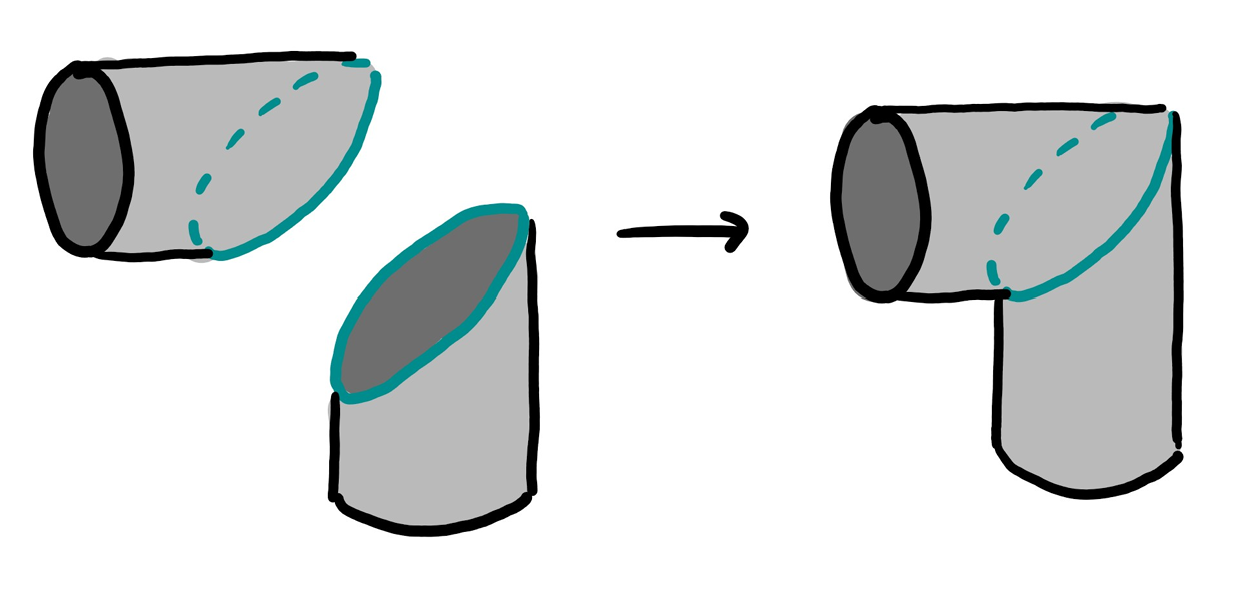
\includegraphics[width=\textwidth]{images/problemglueing.png}
  \caption{Glueing topologically doesn't give smoothness}
\end{minipage}
\end{figure}
\end{frame}

\begin{frame}{Glueing along Boundary: The Solution}
\begin{figure}
\begin{minipage}[b]{0.9\linewidth}
  \centering
  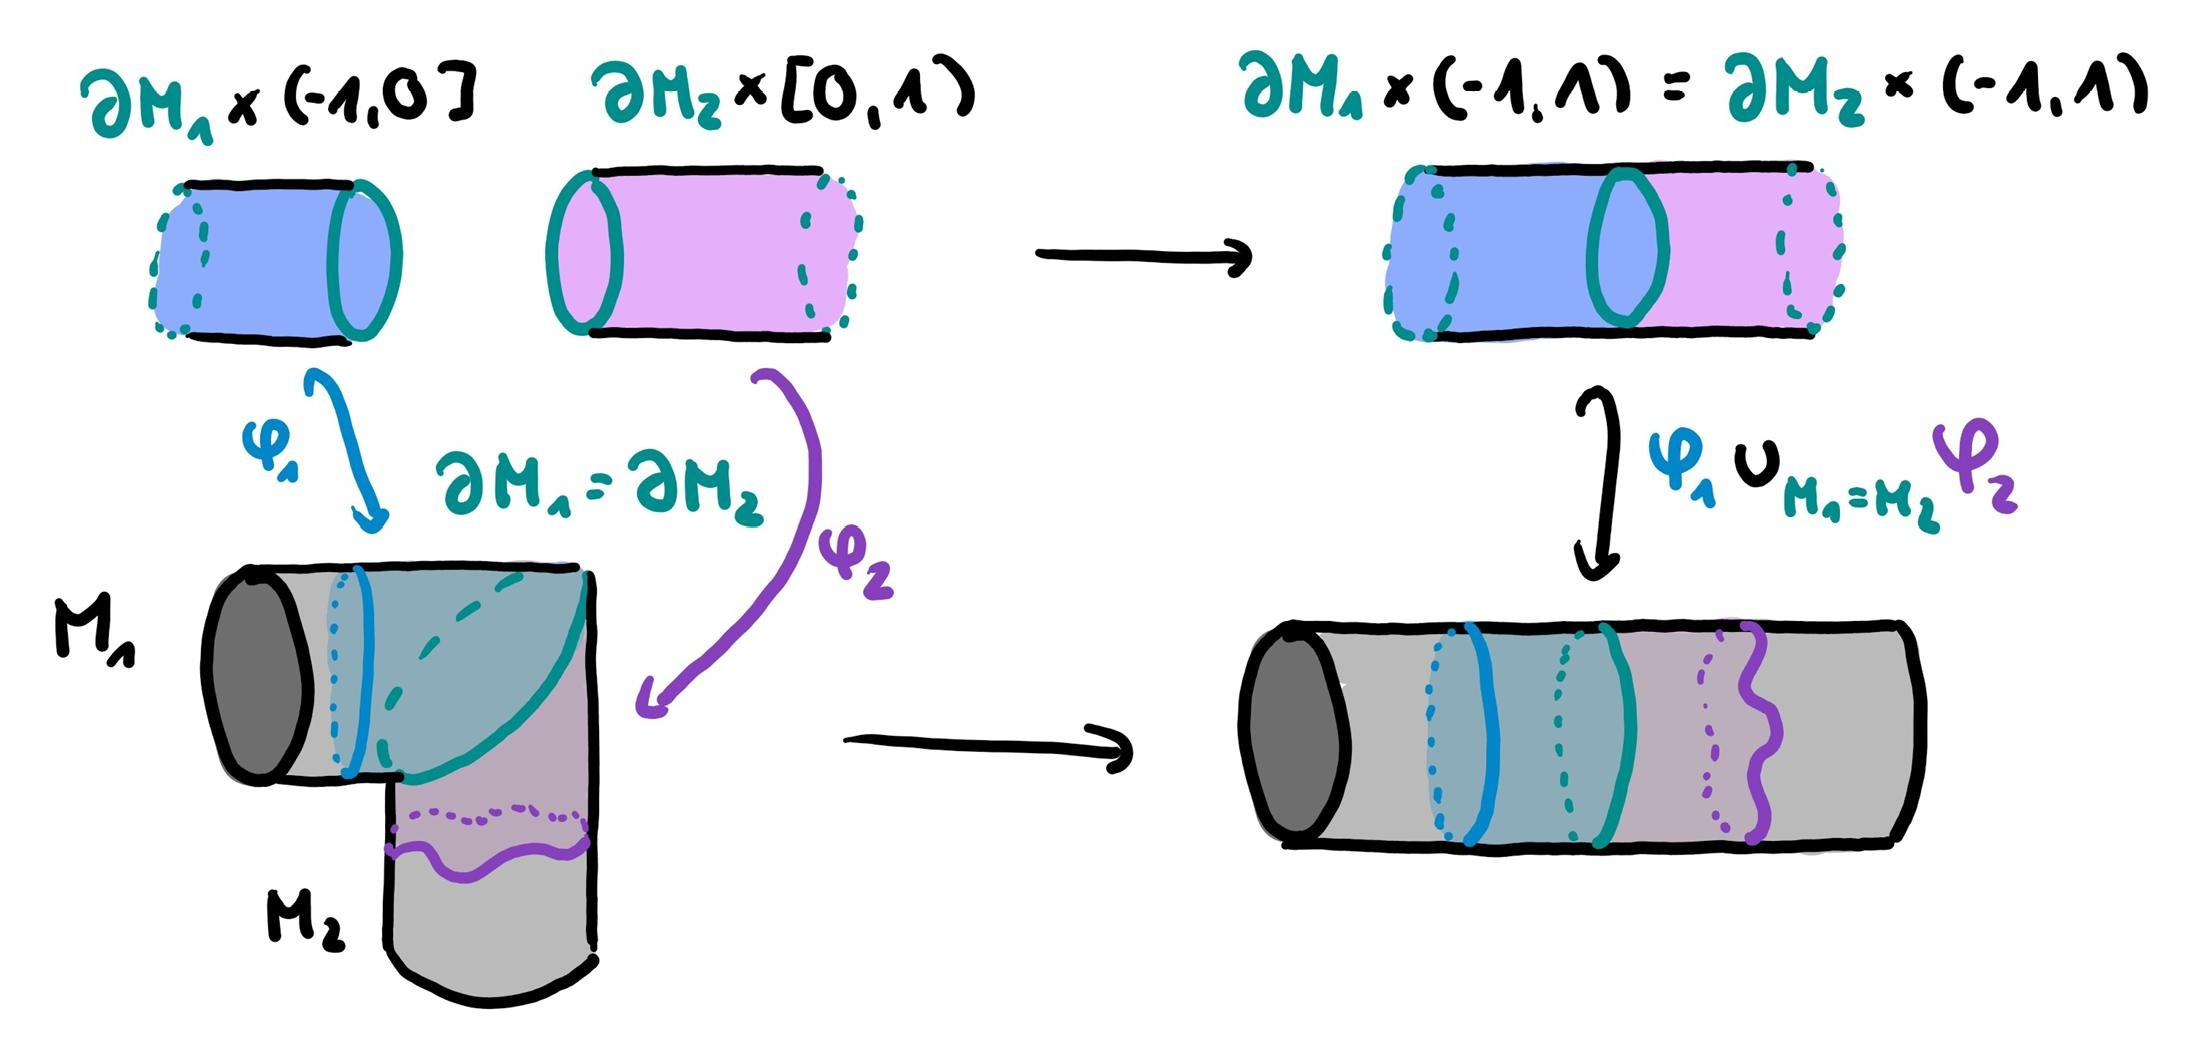
\includegraphics[width=\textwidth]{images/solutionglueing.jpeg}
  \caption{Collar neighbourhoods allow us to define a smooth structure}
\end{minipage}
\end{figure}
\end{frame}

\section{Understanding the Proof}

\begin{frame}{Tangent Bundles}
\setbeamertemplate{enumerate items}[default]
\begin{block}{Definition: Derivation}
A \emph{derivation} at a point $p$ in a smooth manifold with boundary is a linear map $v \colon \smoothfunc{M} \to \bR$ if for all $f, g \in \smoothfunc{M}$ we have $v(fg) = f(p)v(g) + v(f)g(p)$.
\end{block}
\begin{block}{Definition: Tangent Space}
\begin{enumerate}[(i)]
  \item We denote the set of all derivations at $p \in M$ as $\tanspace{p}{M}$ and call it the \emph{tangent space} to $M$ at $p$.
  \item The \emph{tangent bundle} of $M$ is the disjoint union of the tangent spaces at all points of $M$: $\tanbun{M} \coloneqq \coprod_{p \in M} \tanspace{p}{M}$.
\end{enumerate}
\end{block}
\end{frame}

\begin{frame}{Tangent Bundle}
\begin{figure}
  \begin{minipage}[b]{0.4\linewidth}
      \centering
      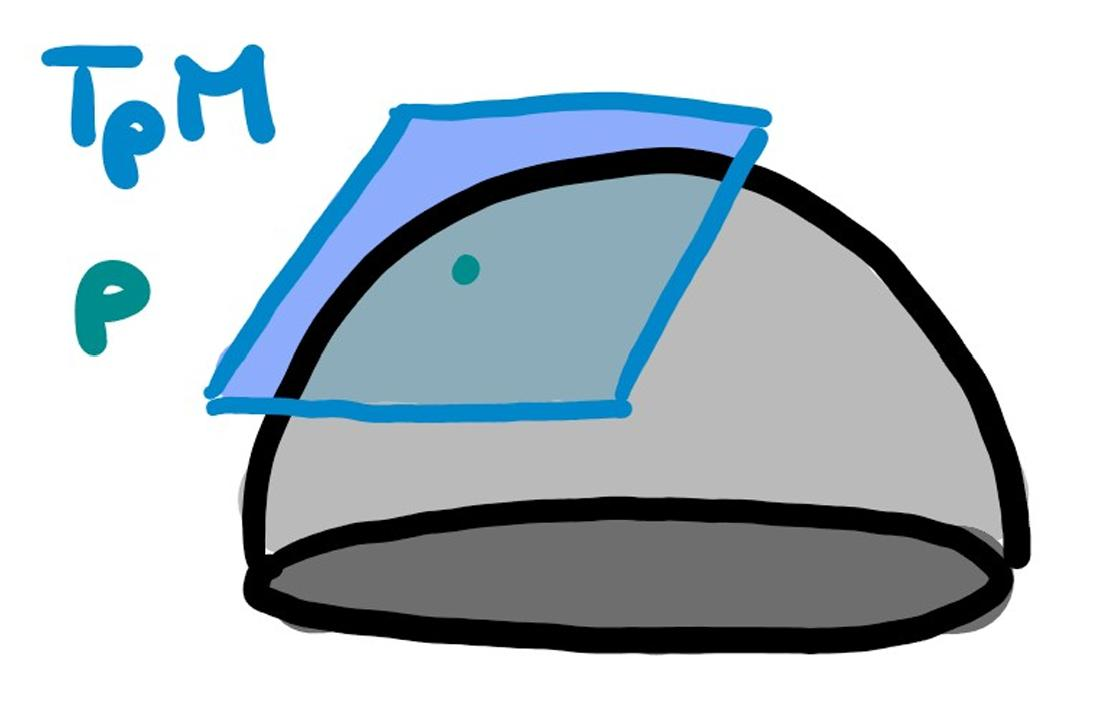
\includegraphics[width=\textwidth]{images/tangentspace.png}
      \caption{Tangent space $\tanspace{p}{M}$ at $p$}
  \end{minipage}
  \hspace{1cm}
  \begin{minipage}[b]{0.4\linewidth}
      \centering
      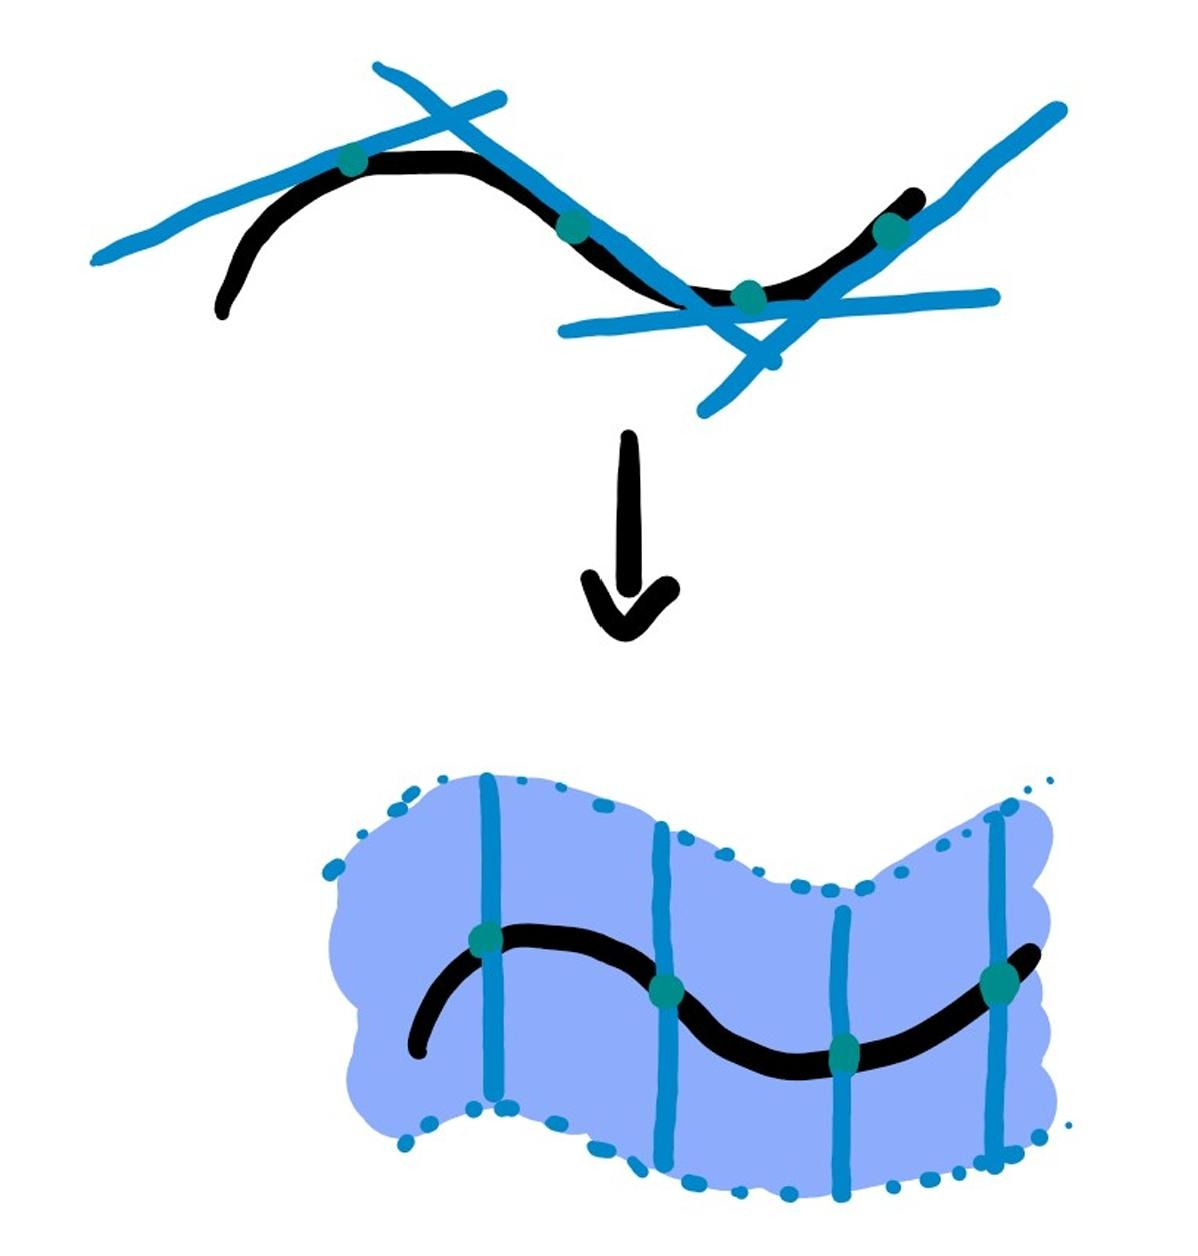
\includegraphics[width=\textwidth]{images/tangentbundle.jpeg}
      \caption{Tangent bundle $\tanbun{M}$}
  \end{minipage}
\end{figure}
\end{frame}

\begin{frame}{Vector field}
\begin{block}{Definition: Smooth vector field}
Let $M$ be a smooth manifold. 
Then a \emph{smooth vector field} on $M$ is a smooth map $X \colon M \to \tanbun{M}$ such that for every $p \in M$, $X(p) \in \tanspace{p}{M}$.
\end{block}
\begin{figure}
\begin{minipage}[b]{0.5\linewidth}
  \centering
  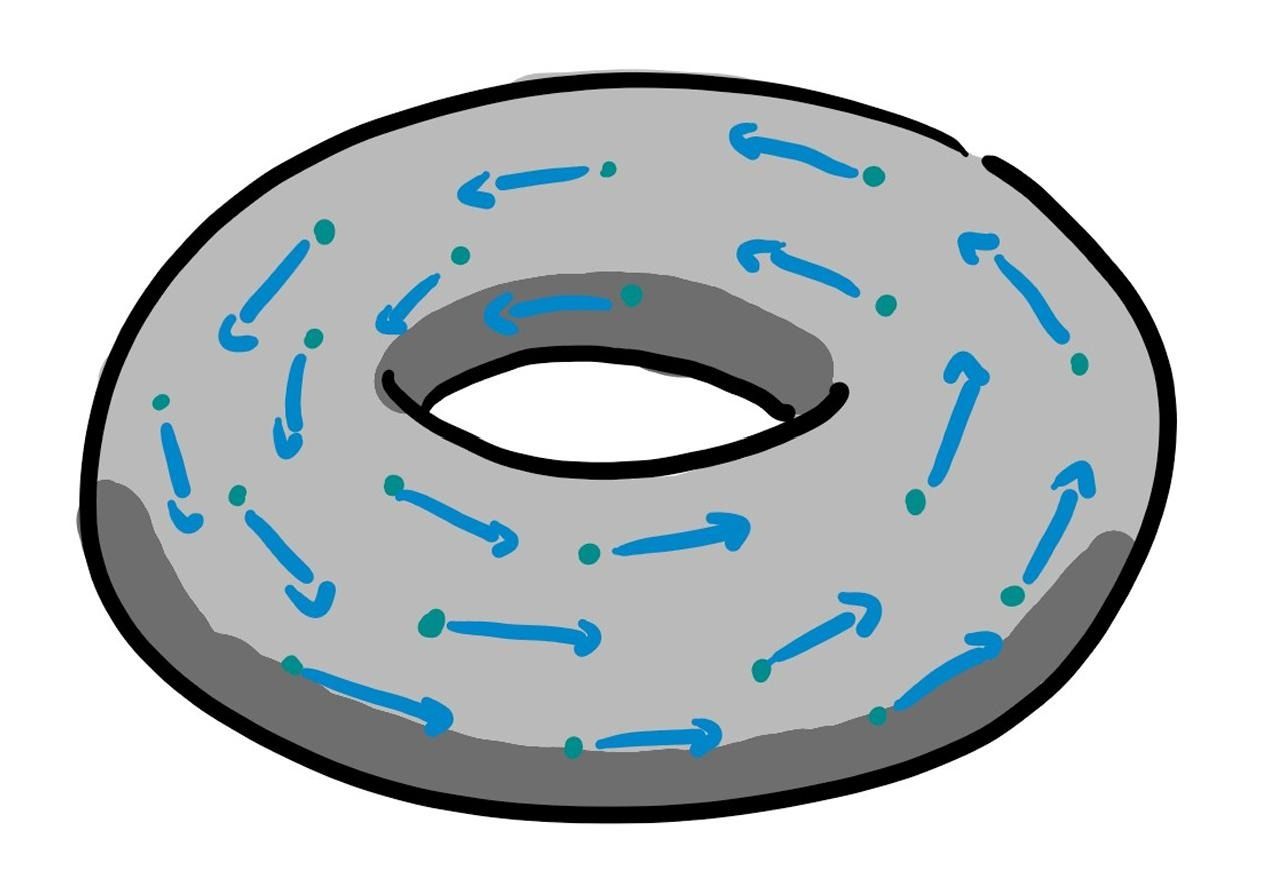
\includegraphics[width=\textwidth]{images/vectorfield.jpeg}
  %\caption{Collar neighbourhoods allow us to define a smooth structure}
\end{minipage}
\end{figure}
\end{frame}

\begin{frame}{Partition of Unity}
\begin{block}{Definition: Partition of Unity}
\setbeamertemplate{enumerate items}[default]
\small
Let $M$ be a topological space and $\fX$ a cover of $M$. 
Then a \emph{partition of unity subordinate to $\fX$} is a family of functions $(\phi_X \colon M \to \bR)_{X \in \fX}$ such that 
\begin{enumerate}[(i)]
  \item $\varphi_X(p) \in [0, 1]$ for all $p \in M$ and $X \in \fX$
  \item $\closure{\{p \in M \mid \varphi_X(p) \ne 0\}} \subseteq X$ for all $X \in \fX$
  \item For every $p \in M$ there is a neighbourhood that intersects only finitely many of $\closure{\{p \in M \mid \varphi_X(p) \ne 0\}}$.
  \item $\sum_{X \in \fX} \varphi_X(p) = 1$ for all $p \in M$.
\end{enumerate}
\end{block}
\end{frame}

\begin{frame}{Partition of Unity}
\begin{figure}
\begin{minipage}[b]{0.6\linewidth}
  \centering
  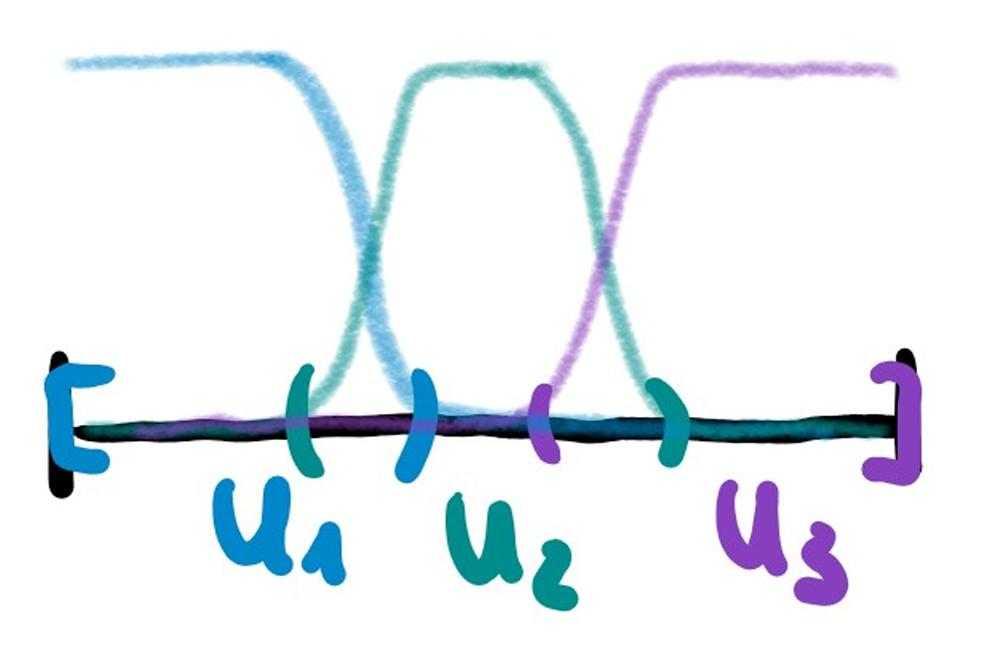
\includegraphics[width=\textwidth]{images/partitionofunity.png}
  \caption{A partition of unity}
\end{minipage}
\end{figure}
\end{frame}

\begin{frame}{Collar Neighbourhoods}
\begin{figure}
\begin{minipage}[b]{0.9\linewidth}
  \centering
  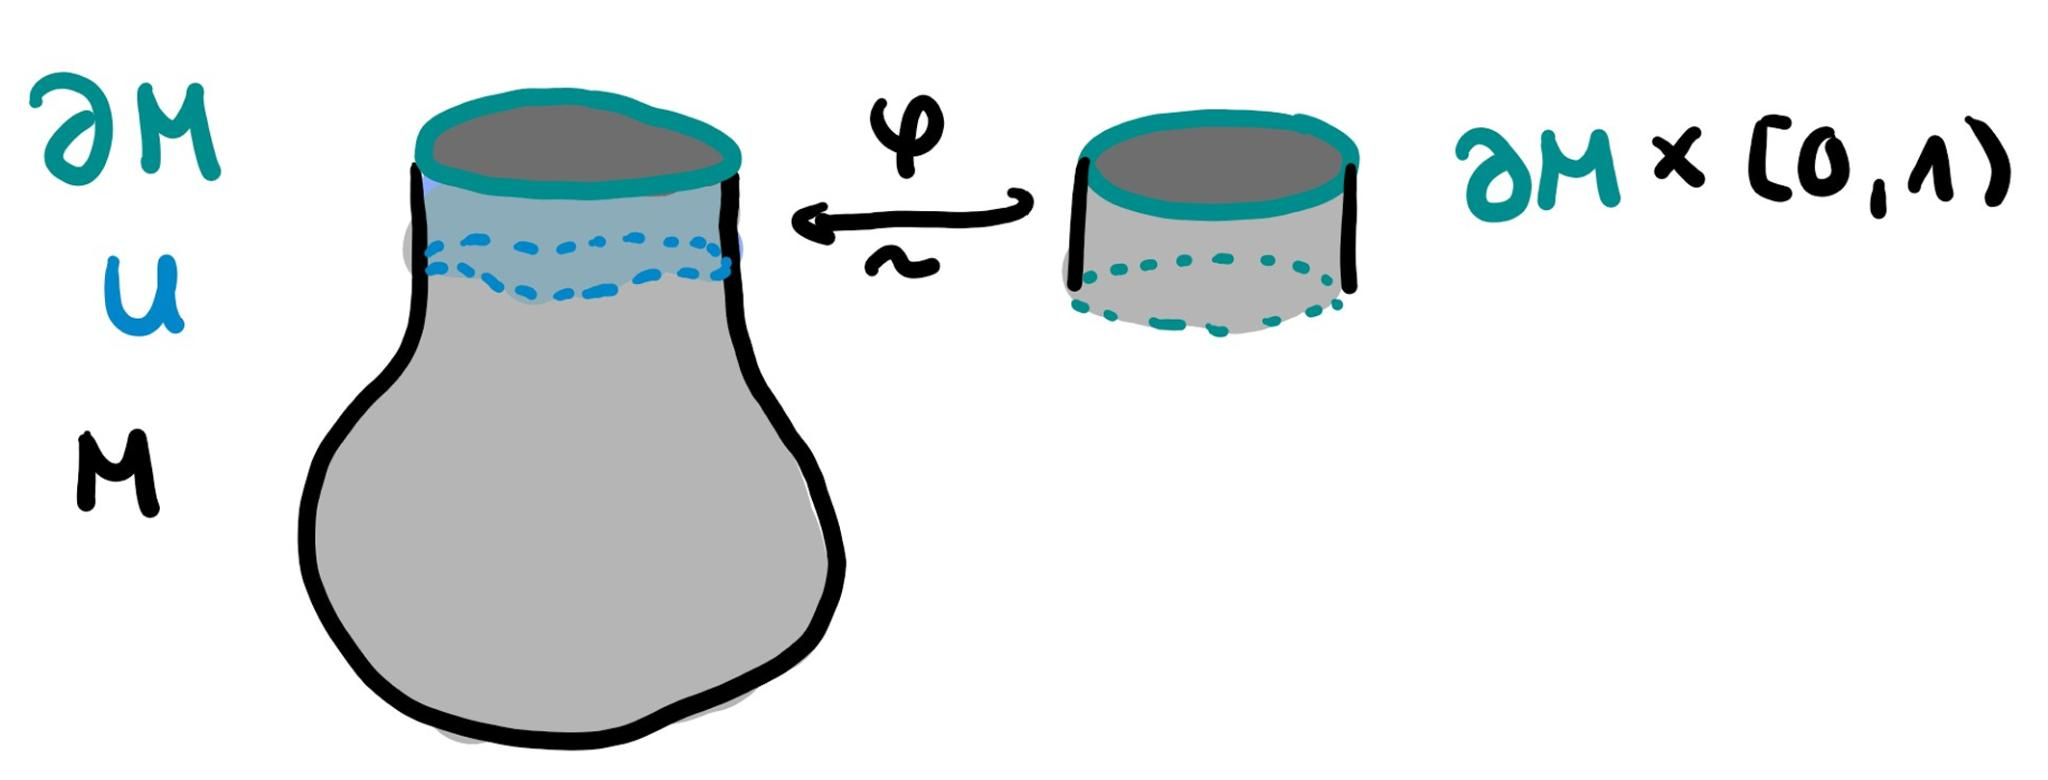
\includegraphics[width=\textwidth]{images/collarneighborhood.png}
  \caption{A collar neighbourhood}
\end{minipage}
\end{figure}
\end{frame}

\begin{frame}{Proof of the Collar Neighbourhood Theorem}
First Step: Define a vector field that is inward-pointing on the boundary. 
\begin{figure}
\begin{minipage}[b]{0.6\linewidth}
  \centering
  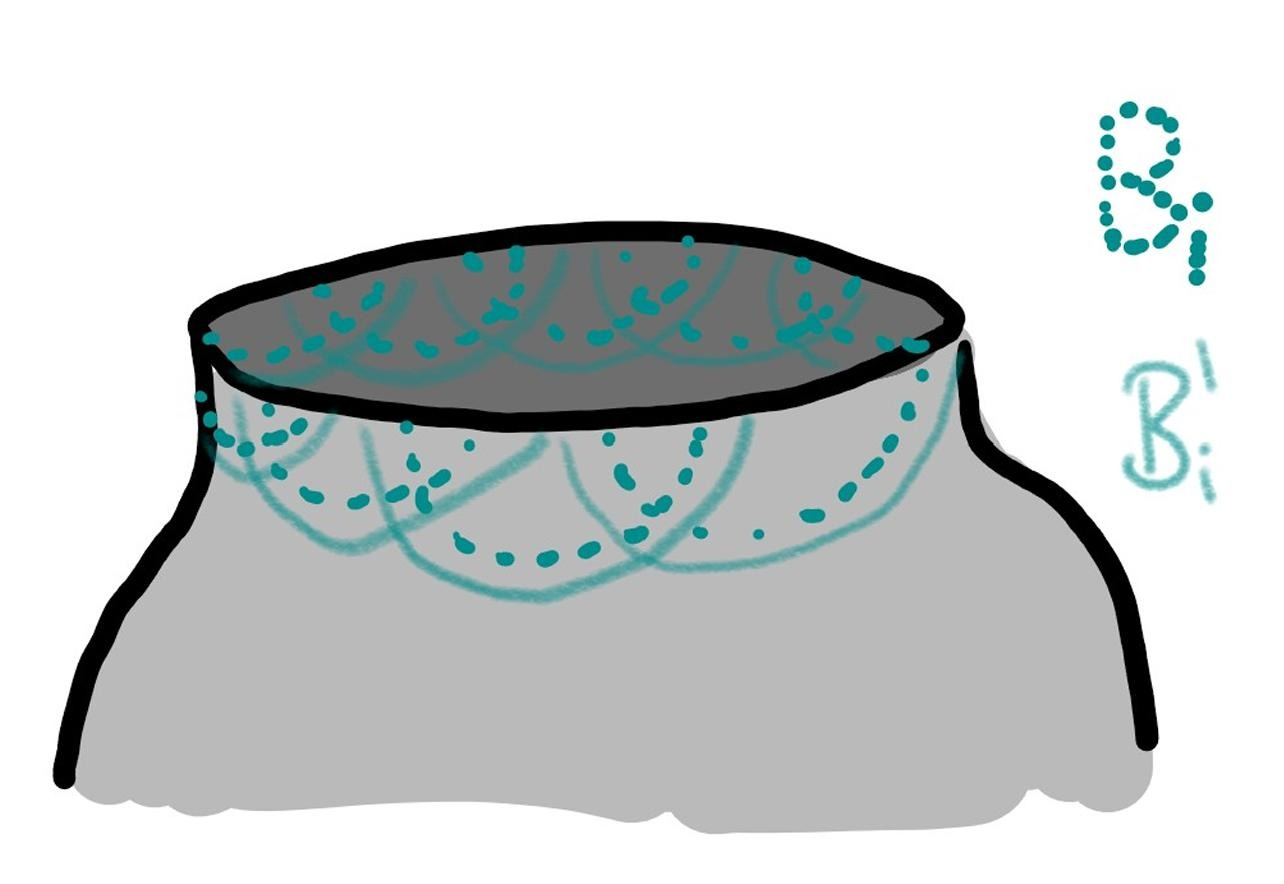
\includegraphics[width=\textwidth]{images/regularcoordinateballs.jpeg}
  \caption{Cover the boundary in regular coordinate half-balls}
\end{minipage}
\end{figure}
\end{frame}

\begin{frame}{Proof of the Collar Neighbourhood Theorem}
First Step: Define a vector field that is inward-pointing on the boundary. 
\begin{figure}
\begin{minipage}[b]{1.05\linewidth}
  \centering
  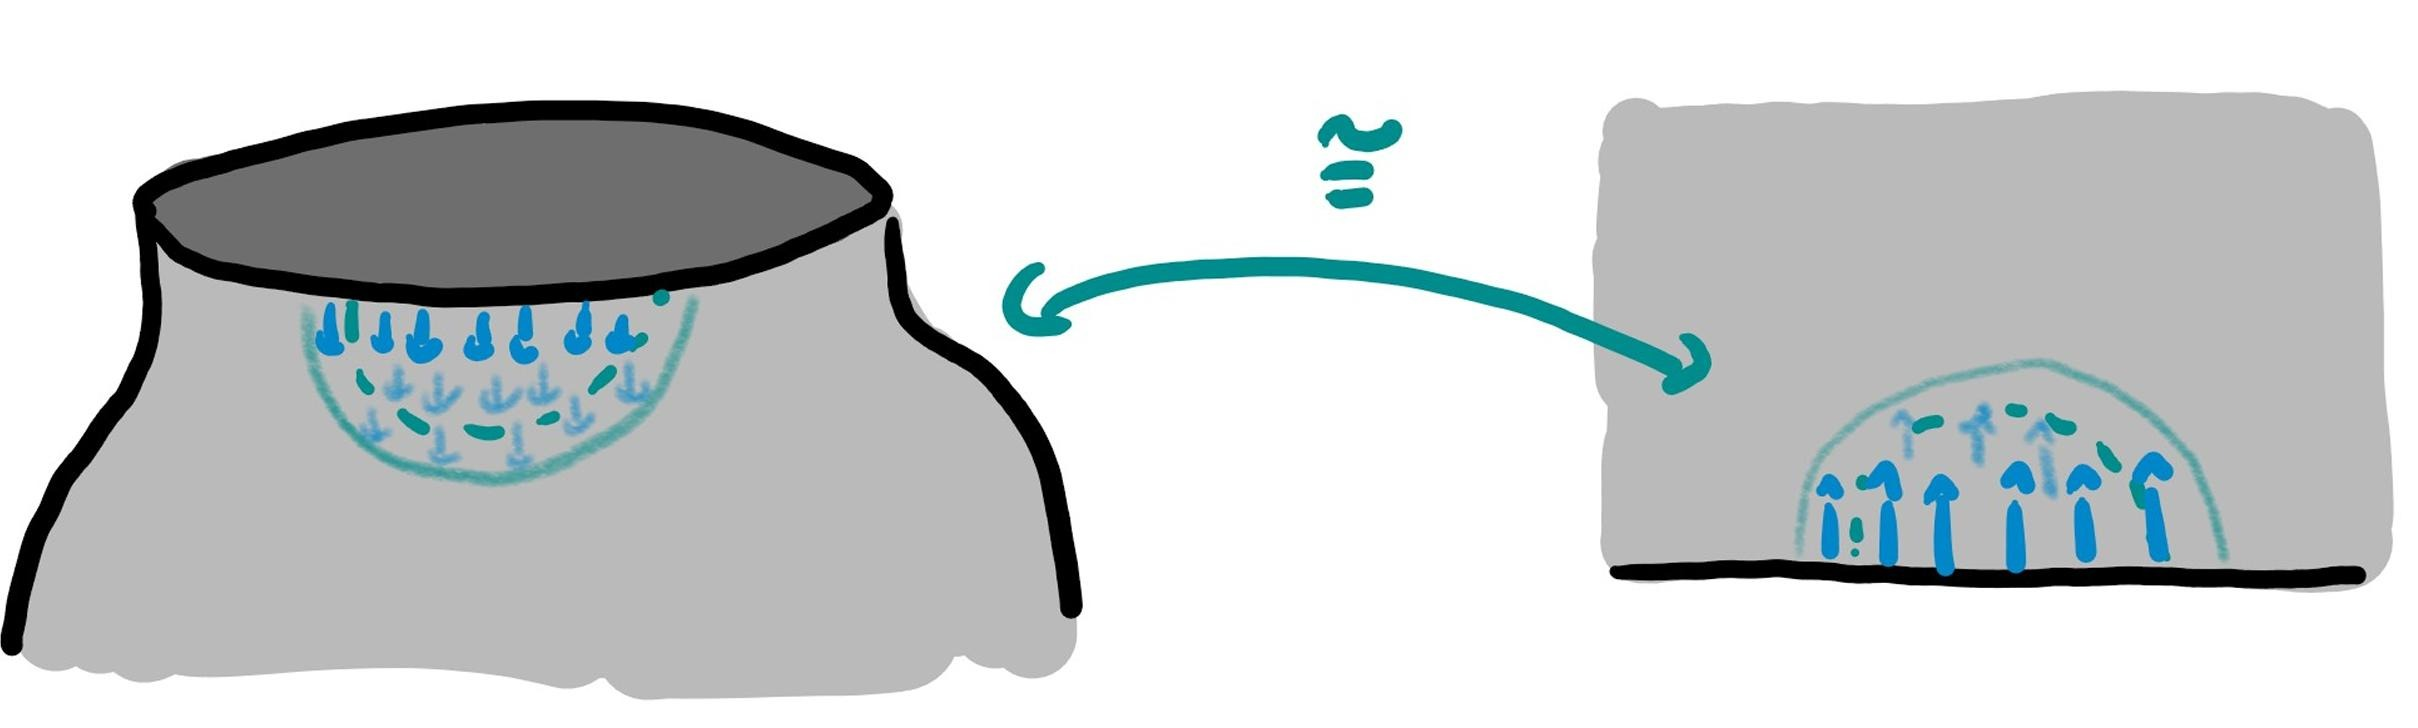
\includegraphics[width=\textwidth]{images/localvectorfield.jpeg}
  \caption{Find a vector field locally}
\end{minipage}
\end{figure}
\end{frame}

\begin{frame}{Proof of the Collar Neighbourhood Theorem}
First Step: Define a vector field that is inward-pointing on the boundary. 
\begin{figure}
\begin{minipage}[b]{0.7\linewidth}
  \centering
  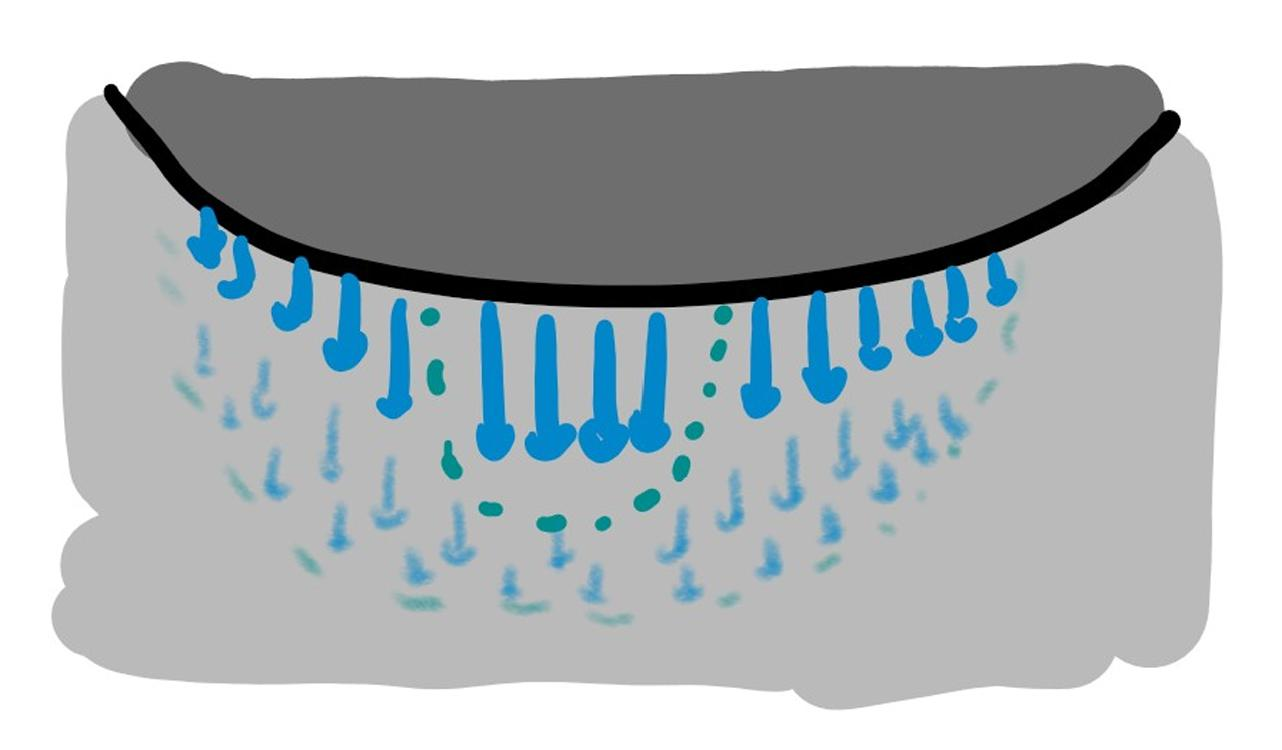
\includegraphics[width=\textwidth]{images/bumpvectorfield.png}
  \caption{Multiply the local vector field with a bump function to extend it into a global vector field}
\end{minipage}
\end{figure}
\end{frame}


\begin{frame}{Proof of the Collar Neighbourhood Theorem}
First Step: Define a vector field that is inward-pointing on the boundary. 
\begin{figure}
\begin{minipage}[b]{0.7\linewidth}
  \centering
  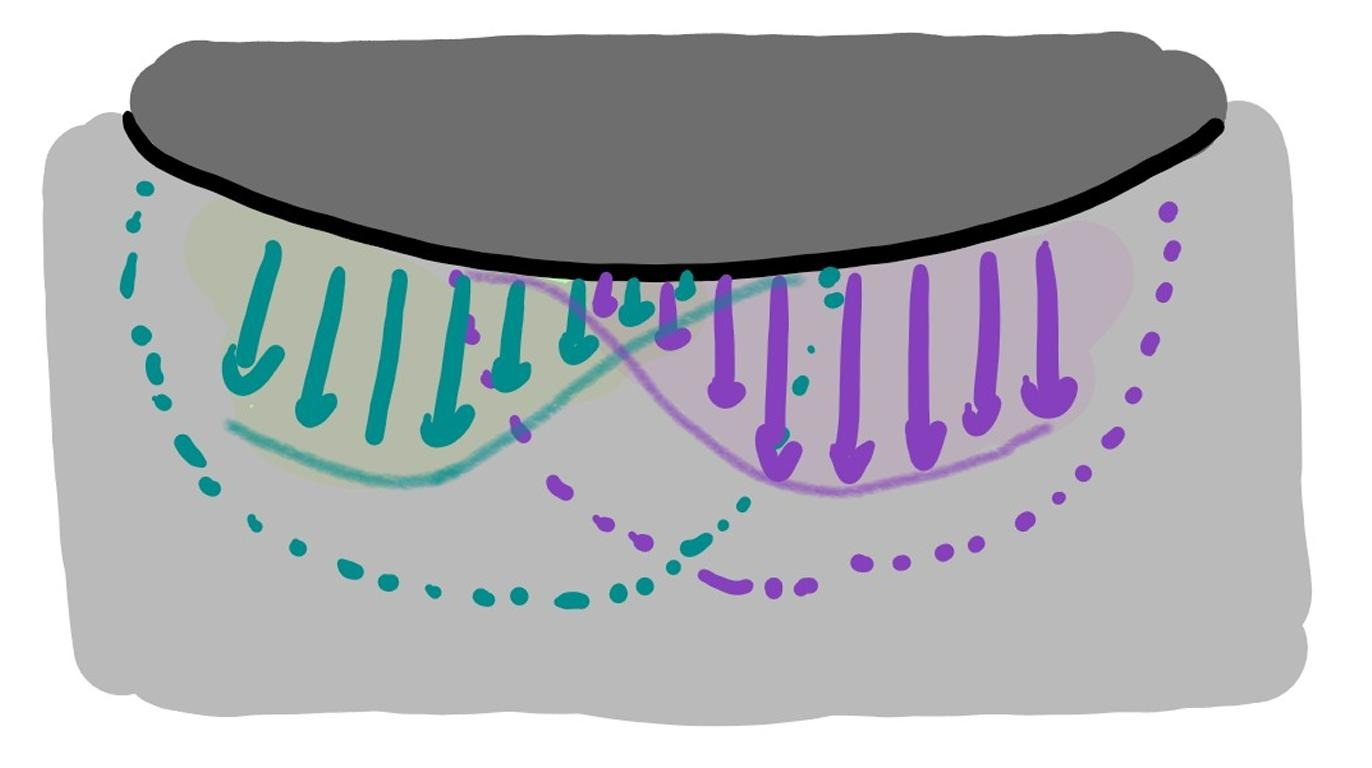
\includegraphics[width=\textwidth]{images/partitionvectorfield.jpeg}
  \caption{Multiply the local vector fields with a partition of untity subordinate to $\{B_i\}_i \cup M \setminus \boundary M$}
\end{minipage}
\end{figure}
\end{frame}

\begin{frame}{Proof of the Collar Neighbourhood Theorem}
First Step: Define a vector field that is inward-pointing on the boundary. 
\begin{figure}
\begin{minipage}[b]{0.7\linewidth}
  \centering
  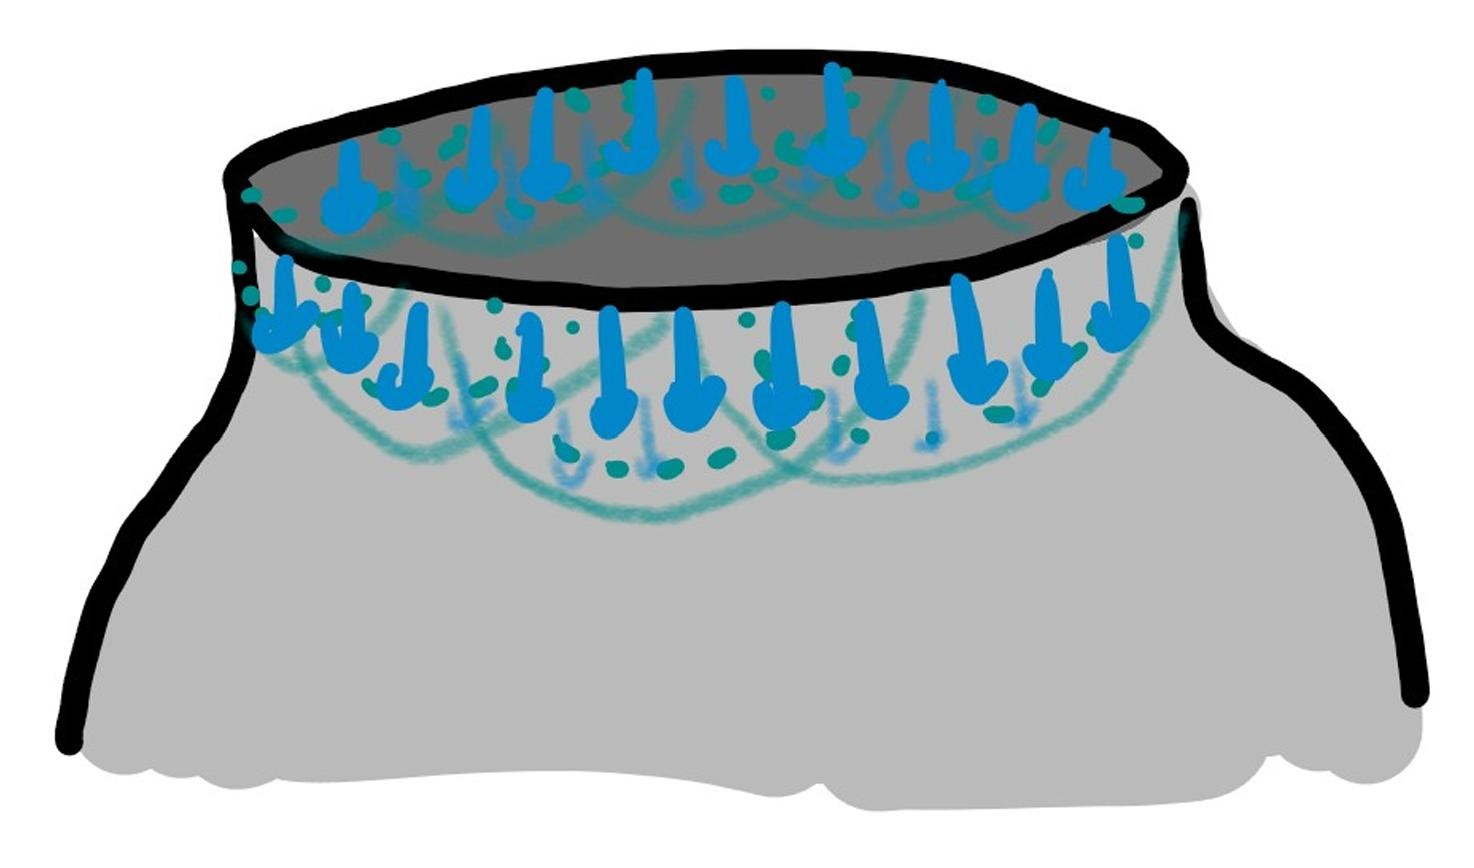
\includegraphics[width=\textwidth]{images/inwardvectorfield.jpeg}
  \caption{Glue together for the desired vector field}
\end{minipage}
\end{figure}
\end{frame}

\begin{frame}{Proof of the Collar Neighbourhood Theorem}
\setbeamertemplate{enumerate items}[default]
Second Step: Apply the Boundary Flowout Theorem. 
\begin{block}{Boundary Flowout Theorem}
Let $M$ be a smooth manifold with non-empty boundary. 
Let $X$ be a smooth vector field on $M$ that is inward-pointing on the boundary. 
Then we obtain: 
\begin{enumerate}[(i)]
  \item A smooth function $\delta \colon \boundary M \to \bR^+$
  \item A smooth embedding $\Phi \colon \fP_\delta \to M$ where $\fP_\delta \coloneqq \{(t, p) \in \bR \times \boundary M \mid 0 \leq t < \delta (p)\}$
\end{enumerate}
such that $\Phi(\fP_\delta)$ is a neighbourhood of $\boundary M$. 
\end{block}
\end{frame}

\begin{frame}{Proof of the Collar Neighbourhood Theorem}
Second Step: Apply the Boundary Flowout Theorem. 
\begin{figure}
\begin{minipage}[b]{\linewidth}
  \centering
  \includegraphics[width=\textwidth]{images/boundaryflowout.png}
  %\caption{Glue together for the desired vector field}
\end{minipage}
\end{figure}

\end{frame}
\begin{frame}{Proof of the Collar Neighbourhood Theorem}
Third Step: Reparametrize $\fP_\delta$.
\begin{figure}
\begin{minipage}[b]{\linewidth}
  \centering
  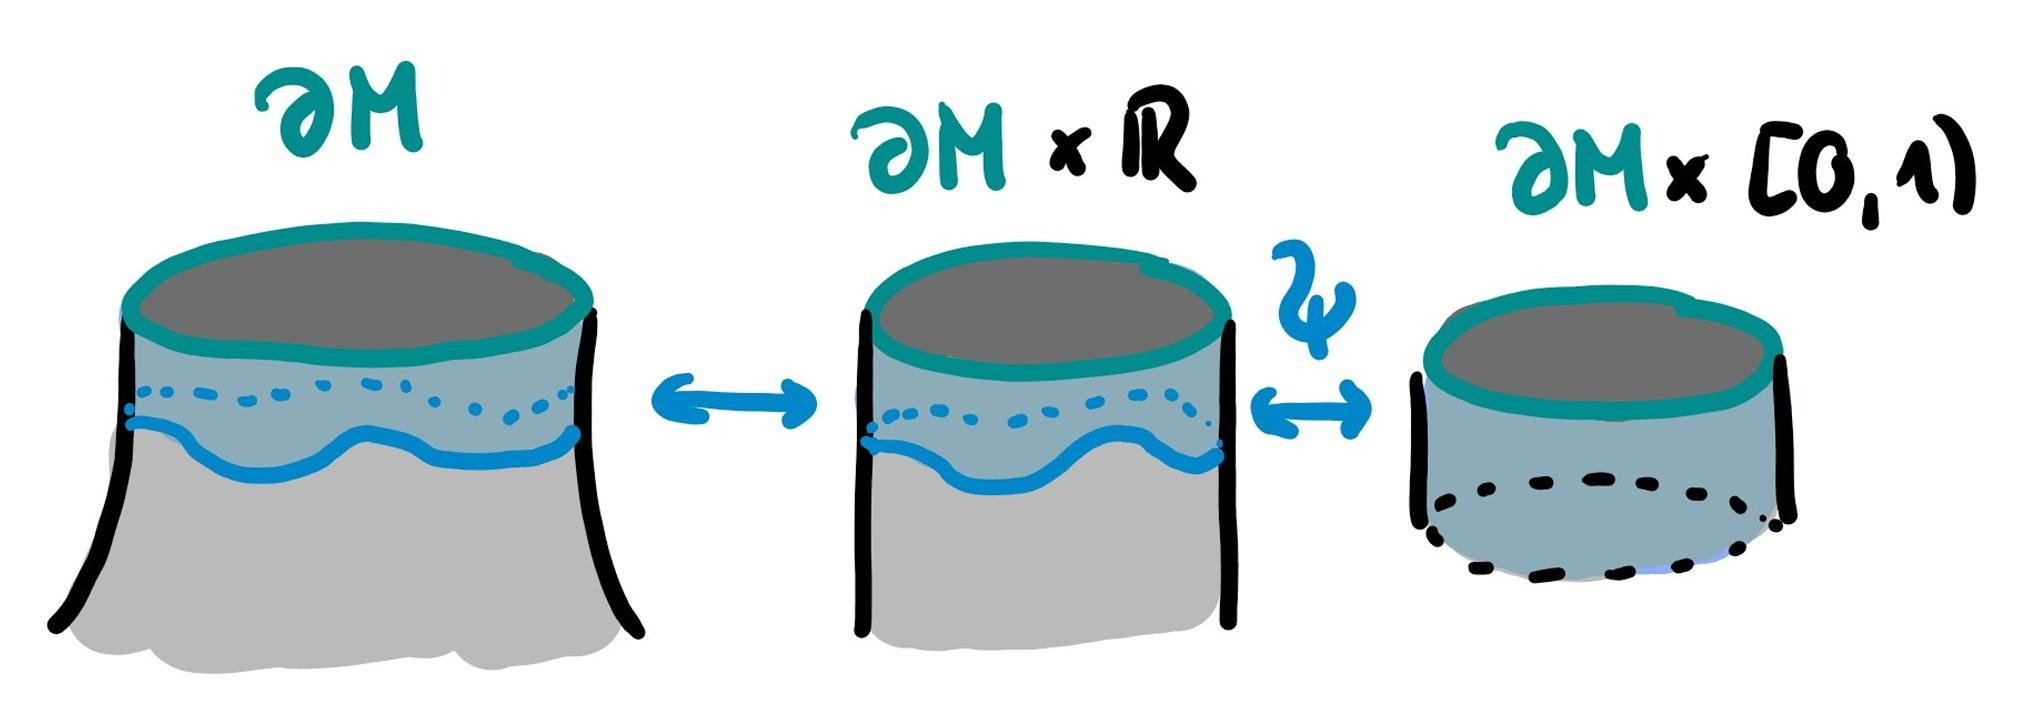
\includegraphics[width=\textwidth]{images/finalproof.png}
  %\caption{Glue together for the desired vector field}
\end{minipage}
\end{figure}
Set $\psi \colon \boundary M \times [0, 1) \to \fP_\delta, (p, t) \mapsto (p, t \delta(t))$.
\end{frame}

\end{document}